
Para el análisis y ajuste se trabajaó con dos conjuntos de datos distintos. El primero fue el conjunto de datos que la colaboración Pierre Auger presentó en la Conferencia Internacional de Rayos Cósmicos (ICRC) del año 2015, este conjunto de datos se utilizó para el cálculo de las correcciones climáticas al estimador de energía \cite{aab2017impact}. El segundo conjunto de datos se presentó en la ICRC del año 2019. Entre estos dos conjuntos de datos existieron cambios en la reconstrucción de energía de los eventos, en particular en el valor de la señal de S$(1000)$ \cite{isabel}, además de agregar la corrección por las modulaciones del clima propuesto en \cite{aab2017impact} sobre este mismo valor de señal y se implementó una función de corte de intesidad constante CIC que varía en función de la energía. El objetivo de este capítulo es comprobar si la corrección del clima de la reconstrucción de eventos es adecuada.

\section{La física detrás de la modulación del clima}\label{seccion:fisica_clima}

El SD mide las 24 horas del día las lluvias de partículas que llegan al suelo. Las señales registradas por los WCDs, ya sea mediante la componente electromagnética o muónica de las EAS, se usan para determinan la posición del núcleo, la dirección de arribo del CR y la energía del primario. La señal de los eventos son ajustados mediante un función de distribución lateral (LDF) para obtener una señal de referencia $S(1000)$. Existieron cambios en los parámetros de la LDF y, por lo tanto, de valor de $S_{38}$, utilizado para estimar la energía del primario. La conversión de $S(1000)$ a $S_{38}$ se realiza mediante el método de corte de intensidad constante (CIC) explicado anteriormente. Además en la nueva reconstrucción el CIC es función de la energía.

\subsection{Trabajos anteriores}

Debido a la modulación del clima dependiente de la estaciones, es de esperarse encontrar una modulación diaria y anual sobre la cantidad de eventos observados por el SD. Ya que en días con menor densidad y presión atmosférica, los tanques detectan eventos por debajo del umbral con mayor facilidad. Este fenómeno fue estudiado por trabajos anteriores realizados por la colaboración Pierre Auger \cite{aab2017impact} \cite{collaboration2009atmospheric}. En particular, el trabajo \cite{aab2017impact} consideró el retraso que tienen los cambios de  la temperatura a distintas alturas sobre la superficie, como se muestra en la Fig\,\ref{fig:delay} que son datos del GDAS (Global Data Assimilation System) promediados por hora del día. Posteriormente esta corrección fue implementada en el proceso  de análisis de datos del observatorio.


En la Fig.\,\ref{fig:delay} se observa que los ajustes realizados a las variaciones de la temperatura  según la hora del día con una función del tipo $T(t) = T_{media} + A\times \sin((t-t_d)\nicefrac{\pi}{12\,\text{hs}})$.  En la Tabla\,\ref{tabla:delay} se observa que entre 1400\,m (altitud del observatorio Pierre Auger) y la mayor altitud medida por el GDAS existe un corrimiento de $2.1\pm0.7\,$hs.

Como la relación entre la densidad y la temperatura del aire están relacionadas mediante la expresión $\rho \approx \nicefrac{0.3484P}{T +273.16}\,$kgm$^{-3}$, con P en hPa y T en  $^o$C \cite{aab2017impact}, el corrimiento de la temperatura al aumentar la altitud también se ve reflejada en la densidad. Como la misma es una variable importante para el desarrollo de la cascada en al atmósfera, este retraso debe tenerse en cuenta.

\begin{figure}[H]
	\centering
	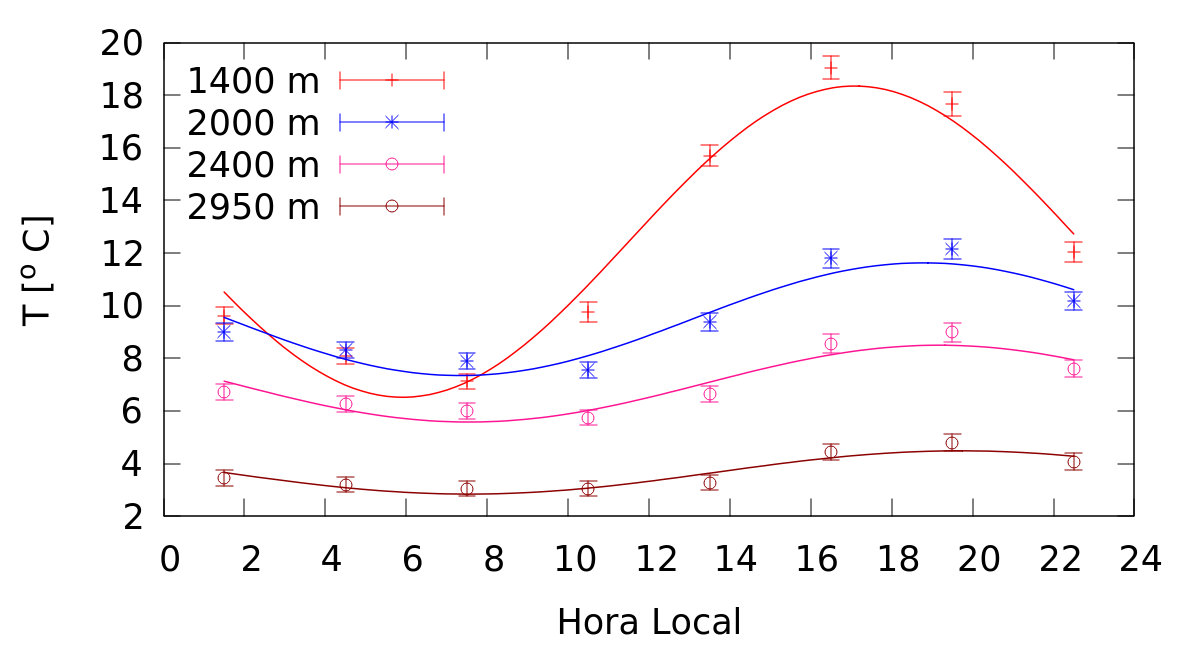
\includegraphics[width=0.65\textwidth]{delay.png}
	\caption{Mediciones de la temperatura a distintas alturas sobre el nivel del mar en función de la hora del día en Malargüe. (Hora Local: UTC-3).}
	\label{fig:delay}
\end{figure}
\begin{table}[H]
\centering
\begin{tabular}{|c|c|c|c|}
\hline
Altura\,[m] & 	T$_{media}$\,[$^o$\,C] 	& A [$^o$\,C] 	& t$_d$ [h] 	\\ \hline
1400		& 	$12.4\pm0.5$			& $5.6\pm0.6$ 	& $12.5\pm0.5$ 		\\ \hline
2000		& 	$9.5\pm0.2$				& $2.1\pm0.3$ 	& $10.8\pm0.6$ 		\\ \hline
2400		&  	$7.0\pm0.2$				& $1.4\pm0.2$	& $10.7\pm0.6$ 		\\ \hline
2950		& 	$3.7\pm0.1$				& $0.8\pm0.1$	& $10.4\pm0.6$ 		\\ \hline
\end{tabular}
\caption{Características de la modulación de la temperatura en función de la altura sobre el nivel del mar.}\label{tabla:delay}
\end{table}

\subsubsection{Efectos de la atmósfera sobre los rayos cósmicos}

La variación de las condiciones atmosféricas afecta las señales de las lluvias atmosféricas extendidas. Estas señales pueden ser detectadas en la superficie por un arreglo de detectores, como los que se encuentran en el Observatorio Pierre Auger. Estos efectos pueden inducir errores sistemáticos en la reconstrucción de energía de los rayos cósmicos. Se han realizado  trabajos anteriores sobre los efectos del clima sobre la señal detectada en el Observatorio Pierre Auger \cite{collaboration2009atmospheric} \cite{aab2017impact}. En este trabajo se estudió eventos con energía mayor a $1\,$EeV entre los años 2005-2018, extendiendo los periodos de tiempo estudiados anteriormente.
%444444444444444444444444444

Para entender los parámetros utilizados para describir a la lluvia, debemos entender que son la longitud de radiación $X_0$, la profundidad de la lluvia $X_{max}$ y el radio de Molière $r_M$. La longitud de radiación definida como $X_0=\nicefrac{d}{2}$,  donde $d$ es un parámetro que indica cuanta cantidad de materia debe atravesar un partícula cargada relativista para perder un factor de $\approx 50\%$ de su  energía. El $X_0$ depende del material que atraviesa la partícula, y tiene unidades de [g\,cm$^{-2}$]. La profundidad de la lluvia $X_{max}$ de una cascada puramente electromagnética, i.e. iniciada por un fotón, tiene la siguiente expresión \cite{matthews2005heitler}
\begin{equation}
 	X_{max} = X_0{ln(\frac{E}{\xi^e_c})}
 \end{equation} 
donde  $\xi^e_c$ es la energía crítica para la cual las pérdida de energía por radiación supera a la pérdidad de energía por colisión, en el aire $\xi^e_c=85\,$MeV. Por último, el radio de Molière $r_M$ que puede expresarse como 
\begin{equation}
	r_M= \frac{E_s}{\xi^e_c}\frac{X_0}{\rho}
\end{equation}
es la máxima profundidad transversal que alcanza la lluvia. El valor de $E_s\approx21\,$MeV caracteriza las pérdidas por dispersión. Usualmente un cilindro con un radio $r_M$ contiene al 90\% de la energía depositada en la atmósfera por el primario. El radio de Molière local en el aire para una altura $h$ puede definirse como $r_M = \nicefrac{9.6\,\text{gcm}^{-2}}{\rho(h)}$ \cite{gora2006universal}. 
%444444444444444444444444444

Las variables atmosféricas importantes que afectan al desarrollo de la EAS en la atmósfera son la presión y la densidad del aire. Por un lado la presión es una medida de cantidad de materia que atraviesa el CR. Si la presión sobre la superficie aumenta implica que la lluvia va a atravesar más partículas, y por el contrario si la presión disminuye la lluvia tiene menos materia para interactuar. Esto afecta el desarrollo longitudinal de la lluvia cuando llega a la superficie. En la Fig.\,\ref{fig:eas} se muestran una esquema simplificado de las interacciones en al atmósfera de un primario de la misma energía. En la figura de la izquierda representa la lluvia donde la presión y la densidad está por encima de la media, y la figura de la derecha representa un lluvia donde la presión y la densidad de la atmósfera están por debajo de la media.

\begin{figure}[H]
	\centering
	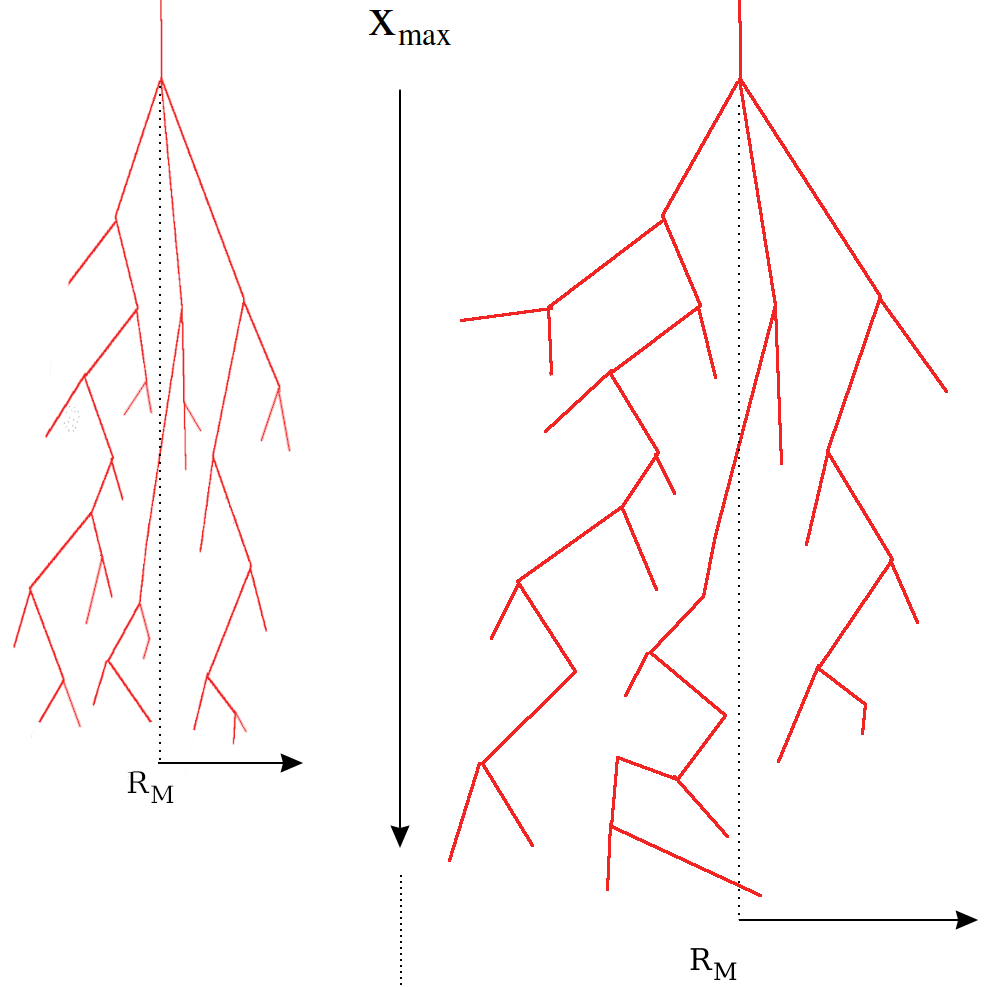
\includegraphics[width=0.5\textwidth]{eas.png}
	\caption{Diagramas simplificado de un lluvia de la misma energía para distintas condiciones atmosféricas}
	\label{fig:eas}
\end{figure}

Estos efectos se ven reflejados en la señal sobre el SD del Observatorio Pierre Auger. La extensión de la señal sobre el SD, es decir el $r_M$ puede cambiar según la densidad de la atmósfera por encima del SD. Los valores de $r_M$ relevantes para la señal medida son a nivel del suelo y a 1000 m. Esto implica que las variaciones de densidad (o de temperatura) a estas alturas están relacionadas con las variaciones al nivel del suelo. La variación a $\sim2400\,$m sobre el nivel del mar está atrasada dos horas con respecto a la variación sobre el Observatorio, que se encuentra a $\sim1400\,$m sobre el nivel del mar. Otro aspecto importante es que la amplitud de está variación disminuye con la altura. Entre las dos altitudes mencionadas existen una relación de aproximadamente $\nicefrac{1}{3}$ entre las amplitudes. 

\subsubsection{Modelo teórico}

Considerando lo analizado en \cite{aab2017impact} \cite{collaboration2009atmospheric}, en este trabajo se propone la siguiente modulación, presentada en la Ec.\,\ref{eq:signal}, para la señal S que reciben los tanques 
\begin{equation}
	S=S_0\big(1+\alpha_P(P-P_0) +\alpha_{\rho}(\rho_{media}-\rho_0) + \beta_{\rho}(\rho_{2h}-\rho_{media})\big)
	\label{eq:signal}
\end{equation}
donde $S_0$ es la señal  del evento en condiciones atmosféricas medias, $P$ es la presión en el momento del evento, $P_0=862\,$hPa es la presión media en el rango de tiempo estudiado, $\rho_{media}$ es la densidad  media del aire en 24\,hs, $\rho_0=1.06\,$kgm$^{-3}$ es la densidad media durante el periodo estudiado, $\rho_{2h}$ es la densidad que se midió dos horas antes del evento  y los coeficientes $\alpha$ y $\beta$ tiene en cuenta la modulación del clima sobre la señal.  Si consideramos la tasa $R_{ang}$  por ángulo sólido $\Omega$

\begin{equation}
	\frac{dR_{ang}}{d\Omega} = \int_{S_{min}}^{\infty} P_{Tr}(S,\theta) d\Phi_{CR}
	\label{eq:rate_angular}
\end{equation}
donde $P_{Tr}$ es la probabilidad de que sea detectado un evento para un valor de señal mínimo $S_{min}$ dado, y $\Phi_{CR}$ es la densidad de eventos por ángulo sólido. La función $P_{Tr}$ tiene en cuenta la eficiencia del disparo de los tanques en función de la energía. Por ejemplo, para el SD 1500 m, como se mencionó anteriormente, la eficiencia máxima de disparo es a partir  de $3\,$EeV. Considerando  las Ecs.\,\ref{eq:s38_energy} y \ref{eq:expresion1} , se puede reescribir la Ec.\ref{eq:rate_angular} como integral de la señal medida S. Teniendo en cuenta que la corrección del clima es pequeña podemos escribir la Ec.\,\ref{eq:signal} como $S=S_0(1+\epsilon)$ y las Ecs. \ref{eq:expresion1} y \ref{eq:s38_energy}.
\begin{align*}
\frac{d\Phi_{CR}}{dE} 	&\propto E^{-\gamma} 					\qquad\qquad\qquad\qquad\qquad \quad \qquad \qquad		\frac{dE}{dS}  			= \frac{dE}{dS_0}\,\frac{dS_0}{dS}\\ 
					  	&= S^{-B\gamma}(1+\epsilon)^{B\gamma}    \qquad\qquad \qquad\qquad\qquad \qquad 				  	 = AB\,S^{B-1}\, (1+\epsilon)^{-B}\\
   		    			\frac{dR_{ang}}{d\Omega} &= \int_{S_{min}}^{\infty} P_{Tr}(S,\theta) \frac{d\Phi_{CR}}{dE} \frac{dE}{dS} dS\\
    						 &\propto \int_{S_{min}}^{\infty} P_{Tr}(S,\theta) \bigg( S^{-B\gamma}(1+\epsilon)^{B\gamma}\bigg) \bigg( AB\,S^{B-1}\, (1+\epsilon)^{-B}\bigg)dS\\
    						 &\propto A\,B (1+\epsilon)^{B\gamma - B}\int_{S_{min}}^{\infty} P_{Tr}(S,\theta) S^{-B\gamma +B -1} dS\\
\end{align*}

Dado que $\epsilon\,\ll\,1$, uno puede expandir la expresión $(1+\epsilon)^{B\gamma}$ hasta primer orden 
\begin{equation*}
	(1+\epsilon)^{B\gamma-B} \approx 1 + B(\gamma-1)\epsilon
\end{equation*}

Por lo que la expresión final queda de la siguiente forma

\begin{equation*}
	\frac{dR_{ang}}{d\Omega} \propto AB(1+B(\gamma - 1)\epsilon)\int_{S_{min}}^{\infty} P_{Tr}(S,\theta) S^{-B\gamma +B -1} dS
\end{equation*}

Considerando que $d\Omega= sin(\theta)d\theta d\phi$ y que el área efectiva  que tiene el observatorio para dado un evento con ángulo cenital $\theta$ es $M_{eff}=M\times cos(\theta)$, donde $M$ es el área activa del observatorio en el momento del evento. Podemos redefinir la tasa por área $R$ como

\begin{align*}
	dR 	&\propto \frac{dR_{ang}}{d\Omega} \frac{M_{eff}}{M} d\Omega \\
		&\propto \frac{dR_{ang}}{d\Omega}\, cos(\theta)\, sin(\theta)\,d\theta d\phi\\
		%&=  AB(1+B(\gamma - 1)\epsilon)\, cos(\theta)\, sin(\theta)\,d\theta d\phi \int_{S_{min}}^{\infty} P_{Tr}(S,\theta) S^{-B\gamma +B -1} dS\\
		&\propto  AB(1+B(\gamma - 1)\epsilon)\,dsin^2\theta d\phi\,\int_{S_{min}}^{\infty} P_{Tr}(S,\theta) S^{-B\gamma +B -1} dS
\end{align*}

Así pudiendo definir la tasa por área por $sin^2(\theta)$, independiente del valor de $\phi$

\begin{align*}
	\frac{dR}{d(sin^2\theta)} &\propto AB(1+B(\gamma-1)\epsilon)\, 2\pi \,\int_{S_{min}}^{\infty} P_{Tr}(S,\theta) S^{-B\gamma +B -1} dS
\end{align*}

Los parámetros $\alpha_P$, $\alpha_{\rho}$ y $\beta_{\rho}$ podrían depender del ángulo cenital o de la energía (por ende de S). En este trabajo se considera solamente la dependencia en $\theta$. Si $P_{Tr}$ es independiente de $\theta$, podemos absorber estas constantes y dejar la expresión como

\begin{equation}
	\frac{dR}{d(sin^2\theta)} = R_0\bigg[1+a_P(P-P_0) +a_{\rho}(\rho_{media}-\rho_0) + b_{\rho}(\rho_{2h}-\rho_{media})\bigg] 
	\label{eq:rate_sin2}
\end{equation}
donde los parámetros $a_P=B(\gamma-1)\alpha_{P}$, $a_{\rho}=B(\gamma-1)\alpha_{\rho}$ y $b_{\rho}=B(\gamma-1)\beta_{\rho}$, donde los parámetros B y $\gamma$ son conocidos.

\subsubsection{Estimador del ajuste}

Para determinar los parámetros del clima, se calcula la tasa de eventos por hora durante un periodo seleccionado normalizada con el área correspondiente a ese momento. Durante el trabajo se menciona la tasa de eventos, pero debe tenerse en cuenta que es la tasa normalizada con el área. Esta área es calculada a partir de la cantidad de hexágonos activos. Por lo tanto, una vez obtenida la tasa, se ajusta la misma mediante la expresión de la Ec.\ref{eq:rate_sin2}, obteniéndose los parámetros del clima.

Para realizar este ajuste, se supone que el número de eventos observado en una hora sigue una distribución de Poisson. Se realiza un ajuste de máxima verosimilitud (\emph{Maximum Likelihood Estimator}) para estimar los coeficientes del clima de la Ec.\ref{eq:rate_sin2}. La función a minimizar tiene la siguiente expresión 
\begin{equation}
	L=\prod_i\frac{\mu_i^{n_i} e^{-\mu_i}}{n_i!}
\end{equation}
donde $\mu_i$ es la media de la distribución de Poisson, que es el número de eventos esperado durante una hora que puede calcularse como
\begin{equation}
	\mu_i = R_0A_iC_i
\end{equation}
donde $R_0$ es la tasa promedio que se observaría si los parámetros atmosféricos fueran los de referencia, es decir $R_0=\nicefrac{\sum n_i}{\sum A_iC_i}$, donde $A_i$ es el área efectiva en el intervalo de tiempo $i$ y el parámetro $C_i$ tiene la forma

\begin{equation}
	C_i = 1+a_P(P-P_0) +a_{\rho}(\rho_{media}-\rho_0) + b_{\rho}(\rho_{2h}-\rho_{media}) 
\end{equation}
con $\rho_{2h}$, como fue mencionado anteriormente, es la densidad medida dos horas antes del evento.

\subsection{Condiciones climáticas y área activa del observatorio Pierre Auger}

Existen tres estaciones meteorológicas dentro del observatorio, que miden cada 5 minutos las condiciones climáticas en distintos puntos. Las ubicaciones de estas estaciones están indicadas en la Fig.\,\ref{fig:auger_sd}. La Fig.\,\ref{fig:clima_p_rho} se muestran las variaciones de los valores de presión y densidad en el periodo del $2005-2018$ con respecto a la media en este mismo periodo. En las mismas se observa las modulación anual de la densidad, Fig.\,\ref{fig:densidad_hora}, y al modulación diaria de la densidad, Fig.\,\ref{fig:area_auger}, que afecta a la detección de las lluvias por parte del SD. 

\begin{figure}[H]
        \begin{subfigure}[b]{0.49\textwidth}
        	\centering
			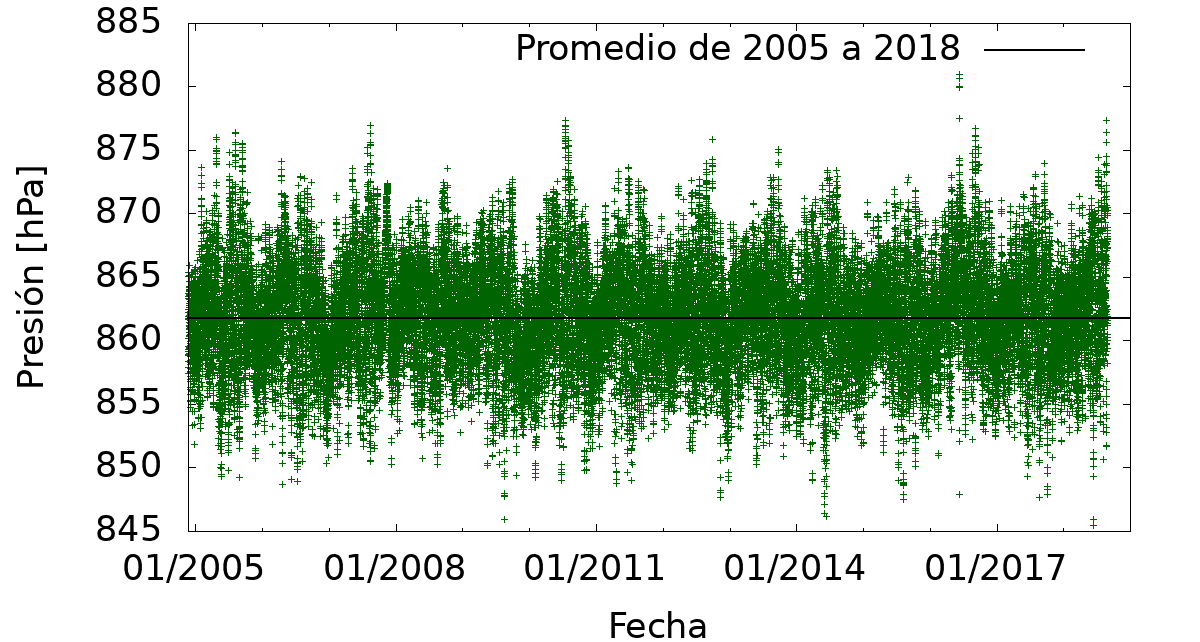
\includegraphics[width=\textwidth]{Graphs/clima/presion.png}
			\caption{Presión}
			\label{fig:presion}
		\end{subfigure}%
		\hspace{\fill}
        \begin{subfigure}[b]{0.49\textwidth}
			\centering	
			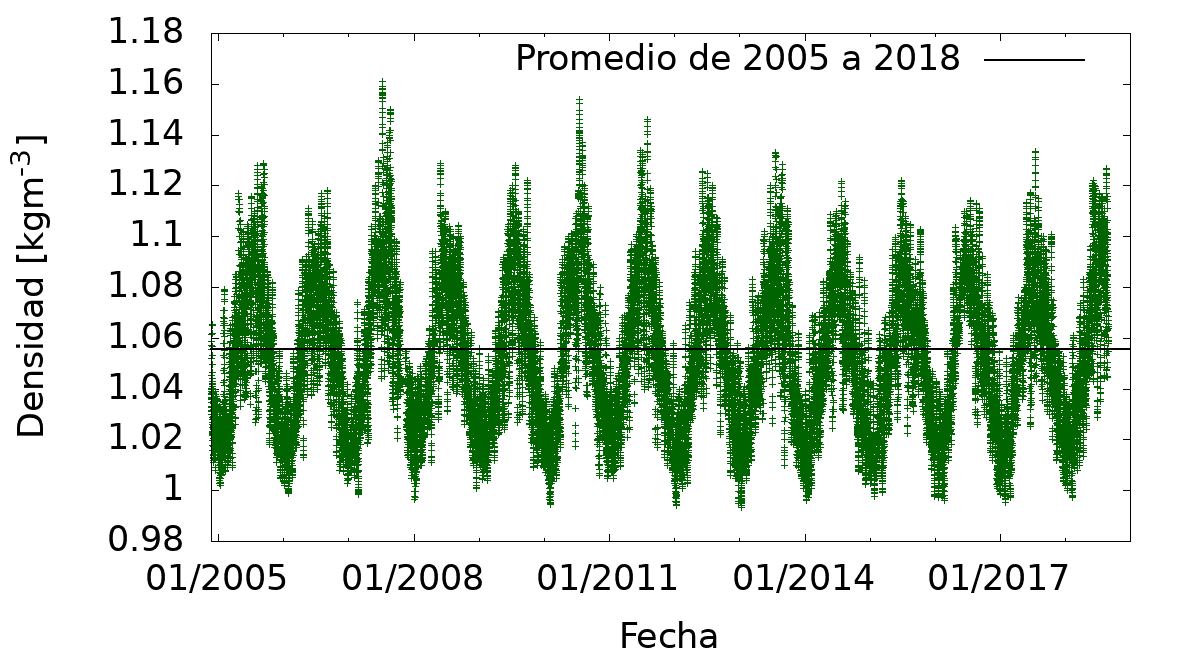
\includegraphics[width=\textwidth]{Graphs/clima/densidad_diaria.png}
			\caption{Densidad diaria}
			\label{fig:densidad_diaria}
        \end{subfigure}%
        \hspace{\fill}
        \begin{subfigure}[b]{0.49\textwidth}
        	\centering
			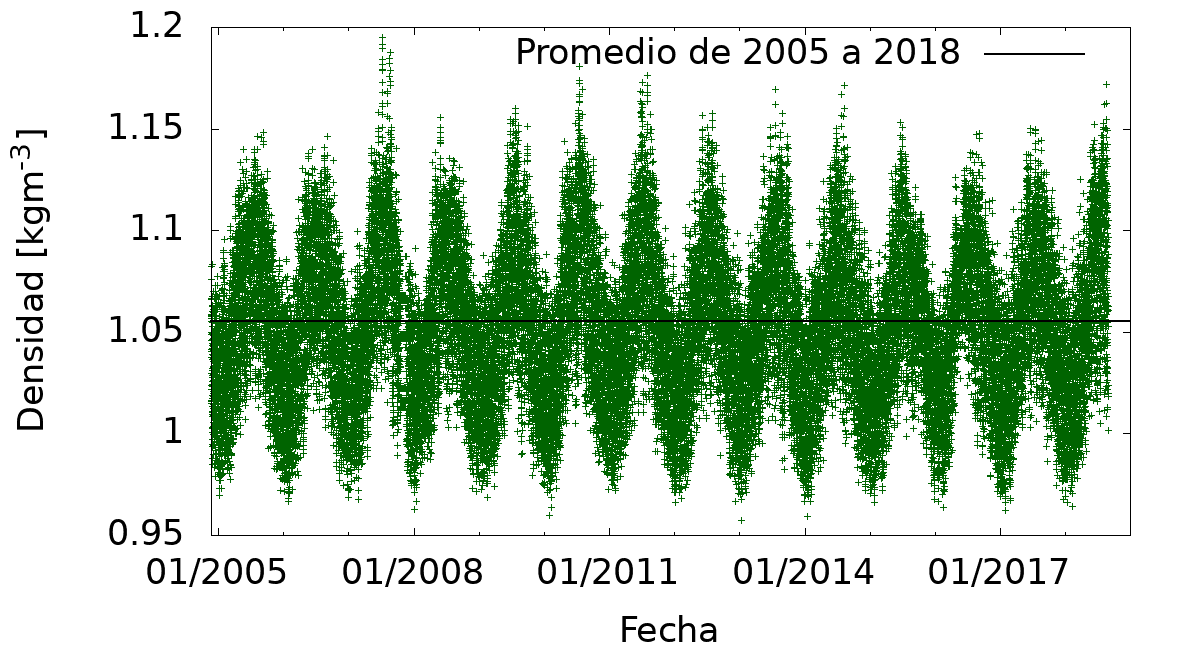
\includegraphics[width=\textwidth]{Graphs/clima/densidad_media_diaria.png}
			\caption{Densidad media por hora}
			\label{fig:densidad_hora}
		\end{subfigure}%
		\hspace{\fill}
        \begin{subfigure}[b]{0.49\textwidth}
			\centering	
			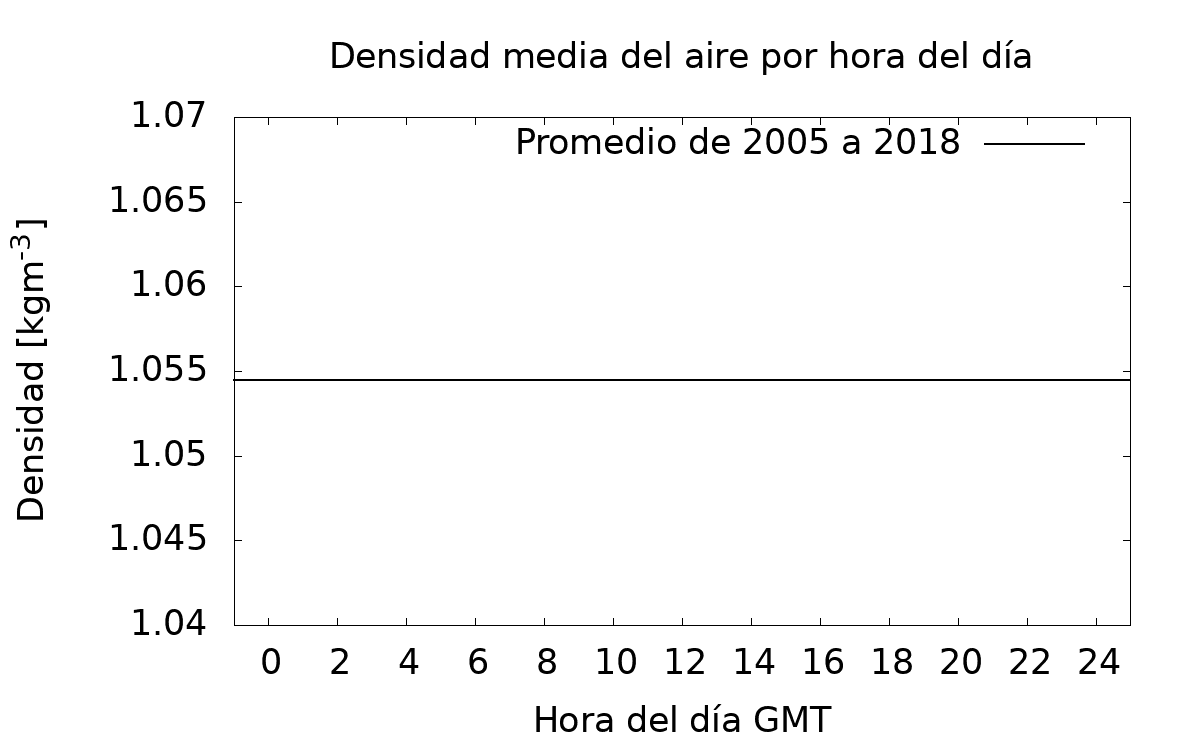
\includegraphics[width=\textwidth]{Graphs/clima/densidad_hod.png}
			\caption{Densidad media por hora del día.}
			\label{fig:area_auger}
        \end{subfigure}%
  \caption{Variaciones de las variables del clima en función del tiempo}
  \label{fig:clima_p_rho}
\end{figure}
